% 页面设置
\documentclass[12pt, a4paper]{article} % 字号:12,纸张:A4
\usepackage[top=2.54cm, bottom=2.54cm, left=3.18cm,right=3.18cm]{geometry} % 页边距设置
% 字体设置
\usepackage[UTF8]{ctex}
\usepackage{fontspec} % 设置字体
%\setCJKmainfont{SimSun}[AutoFakeBold=true, BoldFont={SimHei}, ItalicFont={KaiTi}] % 正文字体
%\setCJKsansfont[AutoFakeBold=3]{KaiTi} % 无衬线字体
%\setCJKmonofont[AutoFakeBold=3]{SimHei} % 等宽字体
\setmainfont{Times New Roman} % 设置主字体为新罗马体
% 文本设置
\usepackage{enumerate} % 支持小标题编号
\linespread{1.5} % 行间距1.5倍
\usepackage{indentfirst}%首段缩进
\setlength{\parindent}{2em} % 首行缩进两字符
\usepackage[hidelinks]{hyperref} % 目录添加超链接
\usepackage{zhnumber} % 章节标题中文显示
\usepackage[cmyk]{xcolor} % 文字彩色显示
% 数学支持
\usepackage{amsmath} % 数学公式支持
\usepackage{amssymb} % 数学符号支持
\usepackage{bm} % 公式加粗
\usepackage{mathrsfs} % 花体字母
\usepackage{yhmath} % 更多的数学符号
% 图片设置
\usepackage{caption} % 插入图片标题
\usepackage{float} % 控制图片位置
\usepackage{subfigure} % 图片并排
\usepackage{booktabs} % 插入表格
% 表格设置
\usepackage{multirow} % 表格自动换行
\usepackage{bigstrut} % 表格间距
\usepackage{rotating} % 表格旋转
\usepackage{tabularx} % 表格宽度
\usepackage{colortbl} % 表格颜色
\usepackage{graphicx} % 表格自动宽度

\title{第六章 \ \ \ 支持向量机} % 文章标题
\author{Castor Ye} % 文章作者
\date{} % 文章时间

\begin{document} % 文档从这里开始。
\maketitle % 按照预定的模板把上面那些信息排好。
\newtheorem{definition}{定义}[section]
\newtheorem{theorem}{定理}[section]
\newtheorem{example}{例}[section]
\newtheorem{solution}{题解}
\newtheorem{algorithm}{算法}
\newtheorem{axiom}{公理}
\newtheorem{property}{性质}
\newtheorem{proposition}{命题}
\newtheorem{lemma}{引理}
\newtheorem{corollary}{推论}[section]
\newtheorem{remark}{注解}
\newtheorem{condition}{条件}
\newtheorem{conclusion}{结论}
\newtheorem{assumption}{假设}
\renewcommand{\figurename}{图} % 将图片序号改为图
\renewcommand{\tablename}{表} % 将表格序号改为表
%%%%%%%%%%%%%%%%%%%%%%%%%%%%%%%%%%%%%%%%%%%%%%%%%%%%%%%%%%%%%%%%%%%%%%%
% 文章内容从此开始

支持向量机是一种经典的二分类模型,基本模型定义为特征空间中最大间隔的线性分类器,其学习的优化目标便是间隔最大化,因此支持向量机本身可以转化为一个凸二次规划求解的问题。

\section{间隔与支持向量}

给定训练样本集 $D = \{(x_1, y_1), (x_2, y_2), \cdots, (x_m, y_m)\}, y_i \in \{-1, +1\}$,分类学习最基本的想法就是基于训练集 $D$ 在样本空间中找到一个划分超平面,将不同类别的样本分开。但是能将训练样本分开的超平面可能有很多,应该如何寻找最优超平面呢?

\begin{figure}[H]
    \centering
    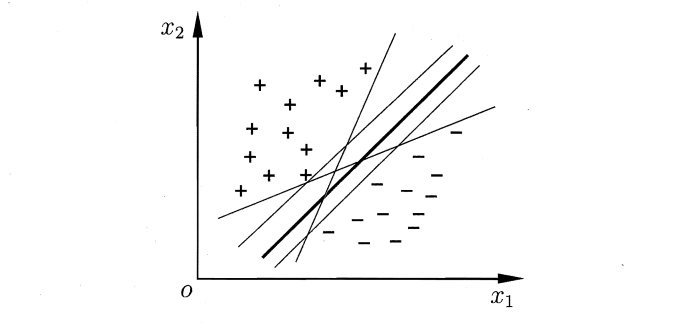
\includegraphics[width=0.8\textwidth]{../img/6-1-存在多个划分超平面将两类训练样本分开.png}
    \caption{存在多个划分超平面将两类训练样本分开}
    \label{fig:存在多个划分超平面将两类训练样本分开}
\end{figure}

直观上看,最优划分超平面所产生的结果是最鲁棒的,对未见示例的泛化能力最强。在样本空间中,我们使用线性方程来描述划分的超平面:
\begin{equation*}
    w^T x + b = 0
\end{equation*}
其中 $w = (w_1;w_2;\cdots;w_d)$ 为法向量,决定了超平面的方向;$b$ 为位移项,决定了超平面与原点之间的距离,我们将其记为 $(w, b)$。

样本空间中任意点 $x$ 到超平面 $(w, b)$ 的距离可写为:
\begin{equation*}
    r = \frac{|w^T x + b|}{||w||}
\end{equation*}

假设超平面 $(w, b)$ 能将训练样本正确分类,即对于 $(x_i, y_i) \in D$,若 $y_i = +1$,则有 $w^T x_i + b > 0$;若 $y_i = -1$,则有 $w^T x_i + b < 0$。令:
\begin{equation*}
    \left\{\begin{matrix}
        w^T x_i + b \ge 1, y_i = +1 \\
        w^T x_i + b \le 1, y_i = -1
    \end{matrix}\right.
\end{equation*}

如下图所示,距离超平面最近的这几个训练样本点使上式等号成立,它们被成为“支持向量”(support vector),两个异类支持向量到超平面距离之和为:
\begin{equation*}
    \gamma = \frac{2}{||w||}
\end{equation*}
它被称为“间隔”(margin)。

\begin{figure}[H]
    \centering
    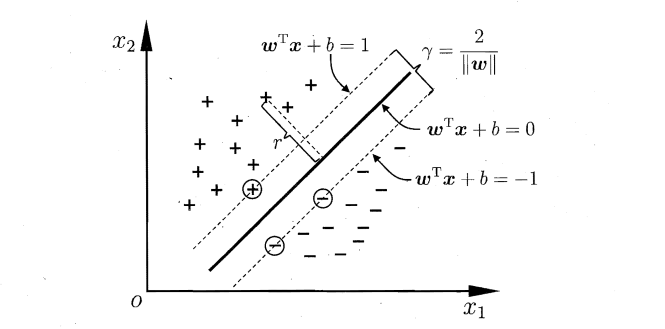
\includegraphics[width=0.8\textwidth]{../img/6-2-支持向量与间隔.png}
    \caption{支持向量与间隔}
    \label{fig:支持向量与间隔}
\end{figure}

欲找到具有“最大间隔”(maximum margin)的划分平面,也就是要找到能满足上式中约束的参数 $w$ 和 $b$,使得 $\gamma$ 最大,即:
\begin{equation*}
    \begin{array}{*{20}{l}}
        \displaystyle \min_{w, b} \frac{2}{||w||}\\
        \displaystyle s.t. \ y_i(w^T x_i + b) \ge 1, i = 1, 2, \cdots, m
    \end{array}
\end{equation*}
这就是支持向量机(Support Vector Machine, SVM)的基本型。

\section{对偶问题}

在上一节中我们得到了一个带约束的凸二次规划问题,我们求解可以得到最大间隔划分超平面所对应的模型:
\begin{equation*}
    f(x) = w^T x + b
\end{equation*}
其中 $w$ 和 $b$ 是模型参数。这个过程可以直接使用现成的优化计算包求解,但我们可以使用更高效的方法。一般我们将原问题变换为它的对偶问题,接着再对其对偶问题进行求解。为什么通过对偶问题进行求解,有下面两个原因:

\begin{enumerate}[\hspace*{2em} i.]
    \item 使用对偶问题更容易求解。
    \item 通过对偶问题求解出现了向量内积的形式,从而能更加自然地引出核函数。
\end{enumerate}

对偶问题,顾名思义,可以理解成优化等价的问题,更一般地,是将一个原始目标函数的最小化转化为它的对偶函数最大化的问题。对于当前的优化问题,首先我们写出它的朗格朗日函数:
\begin{equation*}
    L(w, b, \alpha) = \frac{1}{2} ||w||^2 + \sum_{i = 1}^{m} \alpha_i (1 - y_i(w^T x_i + b))
\end{equation*}
其中 $\alpha = (\alpha_1; \alpha_2; \cdots, \alpha_m$,令 $L(w, b, \alpha)$ 对 $w$ 和 $b$ 的偏导为零可得:
\begin{equation*}
    w = \sum_{i = 1}^{m} \alpha_i y_i x_i, \ \ \ 0 = \sum_{i = 1}^{m} \alpha_i y_i
\end{equation*}

将上式代入,即可将 $L(w, b, \alpha)$ 中的 $w$ 和 $b$ 消去,再考虑其中约束条件,就得到了对偶问题:
\begin{equation*}
    \begin{array}{*{20}{l}}
        \displaystyle \max_{\alpha} \sum_{i = 1}^{m} \alpha_i - \frac{1}{2} \sum_{i = 1}^{m} \sum_{j = 1}^{m} \alpha_i \alpha_j y_i y_j x_i ^T x_j\\
        \displaystyle s.t. \ \sum_{i = 1}^{m} \alpha_i y_i = 0, \alpha_i \ge 0, i = 1, 2, \cdots, m
    \end{array}
\end{equation*}
解出 $\alpha$ 后,求出 $w$ 和 $b$ 即可得到模型:
\begin{equation*}
    f(x) = \sum_{i = 1}^{m} \alpha_i y_i x_i^T x + b
\end{equation*}

其中:
\begin{equation*}
    \begin{array}{*{20}{l}}
        \displaystyle w = \sum_{i = 1}^{m} \alpha_i y_i x_i \\
        \displaystyle b = \frac{
            \displaystyle \max_{i: y_i = -1} w^T x_i + \min_{i: y_i = +1} w^T x_i
        }{2}
    \end{array}
\end{equation*}

从对偶问题解出的 $\alpha_i$ 是拉格朗日乘子,它对应着训练样本 $(x_i, y_i)$。注意到上式中还存在不等式约束,因此上述过程需满足 KKT(Karush-Kuhn-Tucker)条件,即:
\begin{equation*}
    \left\{\begin{matrix}
    \alpha_i \ge 0  \\
    y_i f(x_i) - 1 \ge 0 \\
    \alpha_i (y_i f(x_i) - 1) = 0
    \end{matrix}\right.
\end{equation*}
于是,对任意训练样本 $(x_i, y_i)$,总有 $\alpha_i = 0$ 或 $y_i f(x_i) = 1$。若 $\alpha_i = 0$,则该样本将会在最终模型的求和中出现,也就不会对 $f(x)$ 有任何影响;若 $\alpha_i > 0$,则必有 $y_i f(x_i) = 1$,所对应的样本点对于最大间隔边界上,是一个支持向量。这显示出支持向量机的一个重要性质:训练完成后,大部分的训练样本都不需要保留,最终模型仅与支持向量有关。

对于如何求解出 $\alpha_i$,我们引入SMO(Sequential Minimal Optimization)算法。SMO 的基本思路是先固定 $\alpha_i$ 之外的所有参数,然后求 $\alpha_i$ 上的极值。由于存在约束 $\displaystyle \sum_{i = 1}^{m} \alpha_i y_i = 0$,若固定 $\alpha_i$ 之外的其他变量,则 $\alpha_i$ 可由其他变量导出。于是,SMO 每次选择两个变量 $\alpha_i$ 和 $\alpha_j$,并固定其参数。这样,在参数初始化后,SMO 不断执行如下两个步骤直至收敛:
\begin{enumerate}[\hspace*{2em} i.]
    \item 选取一对需更新的变量 $\alpha_i$ 和 $\alpha_j$。
    \item 固定 $\alpha_i$ 和 $\alpha_j$ 以外的参数,求解模型后获得更新后的 $\alpha_i$ 和 $\alpha+j$。
\end{enumerate}

\section{核函数}

在前面的讨论中,我们假设训练样本是线性可分的,及存在一个划分平面能将训练样本正确分类。然而在现实任务中,原始样本空间内也许并不存在一个能正确划分两类样本的超平面,如下图中的“异或”问题就不是线性可分的:

\begin{figure}[H]
    \centering
    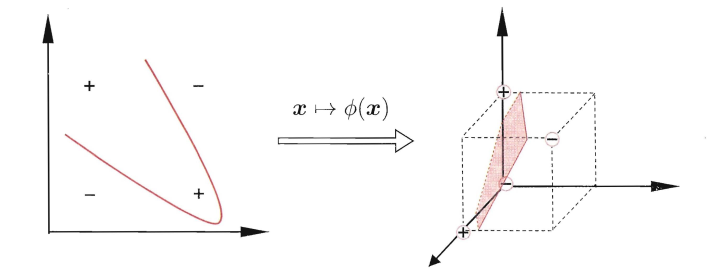
\includegraphics[width=0.8\textwidth]{../img/6-3-异或问题与非线性映射.png}
    \caption{异或问题与非线性映射}
    \label{fig:异或问题与非线性映射}
\end{figure}

对这样的问题,可将样本从原始空间映射到一个更高维的特征空间,使得样本在这个特征空间内线性可分。

令 $\phi (x)$ 表示将 $x$ 映射后的特征向量,于是,在特征空间中划分超平面所对应的模型可表示为:
\begin{equation*}
    f(x) = w^T \phi(x) + b
\end{equation*}
其中 $w$ 和 $b$ 是模型参数,有:
\begin{equation*}
    \begin{array}{*{20}{l}}
        \displaystyle \min_{w, b} \frac{2}{||w||}\\
        \displaystyle s.t. \ y_i(w^T \phi(x_i) + b) \ge 1, i = 1, 2, \cdots, m
    \end{array}
\end{equation*}

则其对偶问题是:
\begin{equation*}
    \begin{array}{*{20}{l}}
        \displaystyle \max_{\alpha} \sum_{i = 1}^{m} \alpha_i - \frac{1}{2} \sum_{i = 1}^{m} \sum_{j = 1}^{m} \alpha_i \alpha_j y_i y_j \phi(x_i) ^T \phi(x_j)\\
        \displaystyle s.t. \ \sum_{i = 1}^{m} \alpha_i y_i = 0, \alpha_i \ge 0, i = 1, 2, \cdots, m
    \end{array}
\end{equation*}

为求解 $\phi(x_i) ^T \phi(x_j)$,我们设想这样一个函数:
\begin{equation*}
    \kappa (x_i, x_j) = <\phi(x_i), \phi(x_j)> = \phi(x_i) ^T \phi(x_j)
\end{equation*}

用该函数重写对偶问题后并求解,得到:
\begin{equation*}
    f(x) = \sum_{i = 1}^{m} \alpha_i y_i \kappa(x, x_i) + b
\end{equation*}



\end{document}